%\documentclass{husttrans}
%\graphicspath{{./}{figure/}}
%
%\usepackage{tcolorbox}
%\usepackage{indentfirst}
%\usepackage{float}
%\usepackage{changepage}
%\usepackage{enumitem,calc}
%
%\title{电子通信系统理论}
%\author{Louis E. Frenzel Jr}
%\translator{王臻哲}
%\supervisor{黑晓军\hspace{1em}副教授}
%\date{2017}{1}{5}
%
%\begin{document}
%
%\frontmatter
%\maketitle

\setcounter{chapter}{1}

%\chapter{电子通信简介}

\chapter{在多智能体群体中产生基础复合语言}
\label{chapter:1}

\section{摘要}

通过在大型语料库中捕获统计模式,机器学习在自然语言处理(包括机器翻译、问答和情感分析)方面取得了显著进展。然而,对于智能地与人类交互的代理来说,仅仅捕获统计模式是不够的。在本文中,我们研究了在多智能体群体中,基础复合语言能否以及如何作为一种手段去实现这个目标。为此,我们提出了一种多智能体的学习环境和学习方法,从而产生了一种基本的复合语言。这种语言被表示为代理随时间发出的抽象离散符号流,但它是具有定义的词汇和语法的一致性的结构。当语言交流不可用时,我们还观察到非语言交流的出现,例如指向和引导。

\section{介绍}

开发能够通信和灵活使用语言的代理是人工智能领域长期面临的挑战之一。如果要成功地作为一个集体进行协调,代理需要发展沟通。此外,代理需要一些语言能力,如果他们要与人类互动并富有成效地协作,或做出人类可以理解的决定。如果这种能力是人为地产生的,它也可以提供关于人类语言和认知发展问题的重要见解。
\par
但是,如果我们希望从第一原则开始形成沟通,那么它必须是必要的。学习从人类语言的例子中合理地模仿语言的方法,虽然非常有用,但却不了解语言存在的原因。这种受监督的方法可以捕获语言中的结构和统计关系,但它们不能捕获其功能方面,或者语言是为了人类之间的成功协调而产生的。在语言合理性的基础上评估这种基于模仿的方法的成功与否也带来了模糊性问题和需要人为参与。
\par
最近,人们对语言使用的实用方面产生了新的兴趣,这也是我们工作的重点。我们采用了(Gauthier和Mordatch 2016)的观点,即当代理人能够使用语言(以及非语言交流或物理行为等其他工具)来实现其环境目标时,他就会对语言有所了解。这导致评估标准可以精确测量而且无需人为参与。
\par
在本文中,我们提出了一个基于物理位置的多智能体学习环境和学习方法,从而引出了一种基本的复合语言。这种语言被表示为代理随时间发出的抽象离散符号流,但它是具有定义的词汇和语法的一致性的结构。代理发出的信号没有任何预先设计的含义,代理只是产生与任务和环境相关的概念,并分配任意符号来传达它们。
\par
类似地,没有明确的语言使用目标,例如正确的话语,并且没有明确的角色代理被分配,例如说话者或听众,或者像传统语言游戏那样的明确的轮流对话结构。可以有任意数量的代理在同时沟通的人群中,其中一些困难是向特定的代理人学习。这些代理就像是位于连续二维环境中的移动粒子,具有诸如颜色和​​形状的特性。代理的目标是以非语言目标为基础的,例如迁移到一个地方,而语言是由协调这些目标的需要而产生的。我们不依赖任何监督,如人为示范或文本语料库。


\section{相关工作}
近年来,在机器翻译等实际自然语言应用方面取得了实质性进展(Sutskever,Vinyals和Le 2014; Bahdanau,Cho和Ben-gio 2014),情感分析(Socher et al.2013),文档摘要(Durrett,Berg-Kirkpatrick和Klein 2016),和特定领域的对话(Dhingra等人,2016年)。许多这种成功的结果是智能设计的统计模型在大型静态数据集上训练的原因。但是,这些方法并不能使机器产生能与人类进行富有成效的合作这种程度的语言理解。
\par
对语言理解的实用主义观点的兴趣长期存在(Austin 1962; Grice 1975),并且最近在(Gauthier和Mordatch 2016; Lake等人2016; Lazaridou,Pham和Baroni 2016)中提出过争论。在双人参考游戏(Golland,Liang和Klein,2010; Vogel等人,2014; Andreas 和 Klein,2016)的背景下提出了语用语言,侧重于通过学习语言识别对象引用的任务。 (Winograd 1973; Wang,Liang和Manning 2016)在物理环境中使用地面语言,并专注于与人类的语言交互,以完成物理环境中的任务。 在这种务实的环境中,空间概念的交流语言使用受到了特别的关注(Steels 1995; Ullman,Xu和Goodman 2016)
\par
除了通过语言生成可以与人类互动的代理人之外,语用语言理解的研究可以扩充我们对语言学和认知科学的认识。这些领域特别感兴趣的问题一直是语法和组成结构是怎么出现的,为什么它在很大程度上是人类独有的语言(Kirby 1999; Nowak,Plotkin和Jansen 2000;Steels2005)。诸如Rational Speech Acts之类的模型(Frank和Goodman 2012)和迭代学习(Kirby,Griffiths,和Smith 2014)已经在认知科学和进化语言学使用地很流行了,但这种方法倾向于依赖预先规定的程序或模式,限制了其一般性。
\par
最近与我们的工作最相似的是强化学习方法应用于学习通信协议的研究,比如(Bratman et al.2010; Foerster et al. 2016; Sukhbaatar,Szlam 和 Fergus 2016; Lazaridou,Peysakhovich 和 Baroni 2016)。


\section{问题的形成}

我们考虑把它设置成一个合作的并且部分可观察的马尔可夫游戏(Littman 1994),它是马尔可夫决策过程的多智能体扩展。它是用由状态集$\mathcal{S}$ 来代表可能的配置,状态是一组行动的集合$\mathcal{A}_1$,...,$\mathcal{A}_N$和一组观察的集合$\mathcal{O}_1$,...,$\mathcal{O}_N$有$\emph{N}$ 个的代理的马尔科夫游戏。
它的初始状态是由分布 $\rho$ : $\emph{S}$ $\mapsto$ [0,1]来决定的。状态转换由函数$\mathcal{T}$ : $\mathcal{S}_1$ $\times$ $\mathcal{A}_1$ $\times$...$\times$ $\mathcal{A}_N$ $\mapsto$ $\mathcal{S}$决定。
对于每一个代理$i$,奖励是有函数$r_{i}$ : $\mathcal{S}$ $\times$ $\mathcal{A}_i$ $\mapsto$ $\mathbb{R}$来给出的,观测是由函数$o_{i}$ : $\mathcal{S}$ $\mapsto$ $\mathcal{O}_i$给出的。
每一个代理$i$使用随机的策略$\pi_{i}$ : $\mathcal{O}_i$ $\times$ $\mathcal{A}_i$ $\mapsto$  [0,1]来选择。
\par
在这项工作中,我们假设所有代理都有相同的行动和观察空间,所有代理都按照相同的政策$\pi$行动并获得共享的奖励。 我们考虑有界(T)设置. 在代理合作社设置情况下,问题就是是找到一个政策使所有代理的预期共享回报最大化,那就可以解决联合最小化问题:
\\
\par
 $\max \limits_{\pi} R(\pi)$, 当$R(\pi) = \mathbb{E}[\sum\limits_{t=0}^T\sum\limits_{i=0}^Nr(s_i^t,a_i^t)]$

\begin{figure}[htb]
	\centering
	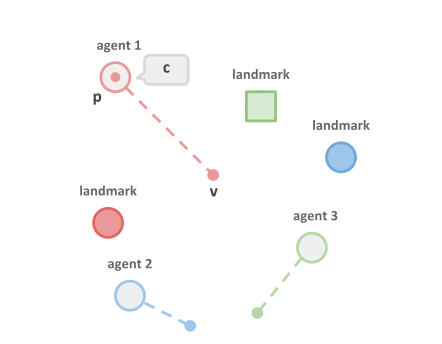
\includegraphics[width=7in]{figure1.png}
	\caption{一个我们认为的环境的例子}\label{fig:环境例子}
\end{figure}

\section{基础通信环境}
正如引言中所论述的那样,物理环境中的基础多代理通信对于产生有趣的通信行为至关重要。在这里,我们考虑在空间连续和时间离散的物理模拟的二维环境。该环境由$\emph{N}$个代理和$\emph{M}$个地标组成。代理和地标实体都位于空间$p$中的物理位置,并且具有描述性的物理特征,例如颜色和形状类型。此外,代理可以将他们的目光引导到一个位置$v$。代理可以在环境中移动并指导他们的凝视,但也可能受到与其他代理人的物理交互的影响。 我们用x表示实体的物理状态(包括描述性特征),并在附录中描述其精确细节和过渡动态。代理可以在环境中移动并直接注意,但也可能受到与其他代理的物理交互的影响。我们用$x$表示一个实体的物理状态(包括描述性特征),并在附录中描述它的精确细节和转换动力学。
\par
除了执行身体动作之外,代理在每个时间节拍都发出口头通信符号$c$。这些符号是大小为$K$的抽象符号词汇$C$的离散元素。我们没有为这些符号指定任何含义。它们被视为抽象的分类变量,由每个代理发出并被所有其他代理商观察。在训练时由代理为这些符号赋予意义。如之前所说,这些
符号被分配给可解释的概念。代理也可以选择在给定的时间步长不发出任何信号,发出信号是一种代价,粗略地代表出通信的更新代价的。我们用粗体$\textbf{c}$表示一个表示符号$c$的独热编码的向量。
\par
每个代理都有独立的向量$\textbf{g}$指定的内部目标,其他代理人不会观察到。这些目标以物理环境为基础,包括例如移动或观测另一个地方任务,这些目标可能会涉及其他代理(例如要求其他代理转移到一个位置,但其他代理没有观察到因此需要代理之间进行协调和沟通。口头言语通信交流是代理之间可以使用的一种工具用于合作完成所有目标,但我们也观察到非语言信号的紧急情况下使用和完全非交际策略的出现。
\par
为了实现这个目标,每个代理都有一个内部循环记忆库$\textbf{m}$,它也是私有的,不会被其他代理观察到。这个内存库没有任何预先设计好的行为,如何正确地使用它完全取决于代理本身。
\par
环境的全部状态是由$s = [\textbf{x}_{1,...(N + M)}\ \textbf{c}_{1,...,N}\ \textbf{m}_{1,...,N}\ g_{1,...,N}  \in \mathcal{S}]$来给出的。每一个代理都会观测到环境中的实体和它们的口头语言通信,以及它们私有的记忆和目标向量。代理$i$的观测就是$\textbf{o}_i(s) = [_{i}\textbf{x}_{1,...,(N+M)}\ \textbf{c}_{1,...,N}\ \textbf{m}_i\ \textbf{g}_i]$。这里的$_{i}\textbf{x}_j$是在代理$i$的参考系下观测到实体$j$的物理状态(具体见附件)。更复杂的观察模型是可能的,例如物理观测仅来自于单个输入通道的像素或口头观察。这些模型将要求代理学习执行视觉处理和源分离,这与我们的工作不相关。虽然观察的维度随着物理实体和通信流的数量不同,如之前所述,我们的策略体系结构允许这些变化。
\begin{figure}[htb]
	\centering
	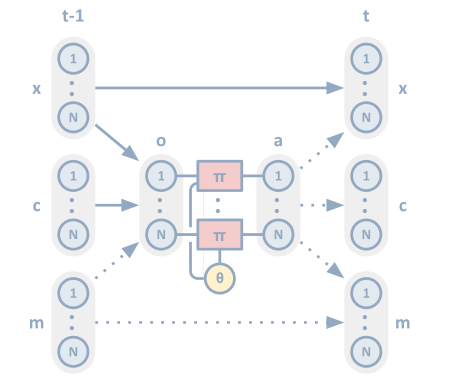
\includegraphics[width=6in]{figure2.png}
	\caption{$N$个代理从时间$t-1$到$t$的动态转变。虚线表示代理之间的一对一依赖关系,实线表示所有依赖项}\label{fig:代理关系}
\end{figure}


\section{基于反向传播的学习策略}
每个代理通过随机策略π对采样动作起作用,该随机策略$\pi$对于所有代理是相同的并且由参数$\theta$定义。有几种常见的查找最优策略政策参数的方法。 $Q-learning$的无模型框架
学习可以用来找到最佳的 状态-动作 ,并根据结果采用贪心策略。 不幸的是,$Q$函数维度与通信词汇量大小成二次关系,这很快变得难以处理。或者,可以使用无模型策略梯度方法直接学习策略函数,该方法使用采样估计策略返回的梯度$\frac{dR}{d\theta}$。 这些方法的梯度估计都有非常高的方差,在通信动作是一个序列的情况下,信用分配成为一个特别困难的问题。
\par 
我们不是使用无模型强化学习方法,而是构建所有代理的端到端可区分模型,环境状态动态随时间变化并用反向传播计算$\frac{dR}{d\theta}$。在每次优化迭代中,我们对一批新的1024个随机环境实例进行抽样,并根据时间反向传播更新它们的动态结果来返回总梯度。图2显示了两个时间节拍之间的依赖关系链。 (Foerster等人2016; Sukhbaatar,Szlam和Fergus 2016)采用了类似的方法来计算通信行为的梯度,尽管后者仍采用无模型方法进行物理行为计算。
\par 
物理状态动态变化,包括不连续关系可以通过平滑来区分。然而,通信行为需要发射离散符号,这给反向传播带来困难。


\section{离散通信和Gumbel-Softmax估计}
为了在我们的设置中使用分类通信排放$\textbf{c}$,必须要能够区分它们。在具有离散变量的可微模型上,机器学习已经有了大量的工作,但是我们发现最近的方法(Jang,Gu和Poole 2016;
Maddison,Mnih和Teh 2016)在我们的环境中特别有效。
该方法提出了Gumbel-Softmax分布,这是一个离散的连续宽松分类分布。 给定 K-种分类 分布
参数为p,来自Gumbel-Softmax分布的可微分K维独热编码样本$G$计算如下:
\par 
$G(log\emph{p})_k = \frac{exp((log\emph{p}_k + \varepsilon) / \tau)}{\sum_{j=0}^k\large exp((logp_j + \varepsilon)/ \tau)}$
\par 
这里的$\varepsilon$是独立同分布的,服从Gumbel(0,1)分布。$\varepsilon = -log(-log(\emph{u})), u \sim \mathcal{U}[0,1]$, $\tau$是一个softmax温度参数。
在所有的训练实验中,我们没有发现有必要对温度进行训练,将其设置为1,直接从分类分布证明时间中取样。为了发出通信符号,我们的策略被训练为直接输出$log\emph{p} \in \mathcal{R}^K$,转换为符号样本就是$\mathbf{c} \sim G(log\emph{p})$。梯度可以估计为$\frac{dc}{d\theta} = \frac{dG}{dp}\frac{dp}{d\theta}$.


\section{策略架构}
我们在这项工作中使用的的策略是随机神经网络。该策略输出物理动作$\mathbf{u}$,符号通信$\mathbf{c}$和内部记忆更新$\Delta\mathbf{m}$的代理的样本。策略必须合并多个代理传入通信符号流好和观察其他物理实体的传入。重要的是,代理的数量(以及跟它有关的通信流的数量)和物理实体的数量可以在环境实例之间变化。
为此,策略为每个通信流实例化一组相同的处理模块,每个观察到的物理实体每个处理模块都是
完全连接的多层感知器。所有通信处理和物理观察模块之间的权重是共享的。各个处理模块的输出与softmax操作合并为特征,矢量$\phi_c$和$\phi_x$分别用于通信和观测物理流。这种权重共享和池化使得可以将相同的策略参数应用于任何数量的通信和物理观察。
\begin{figure}[htb]
	\centering
	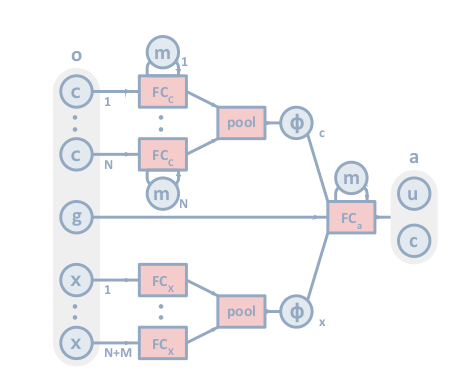
\includegraphics[width=6in]{figure3.png}
	\caption{我们的策略体系结构概述,将观察结果映射到每个时间点的操作。 FC表示与之共享权重和所有其他标签的全连接网络。 pool表示softmax池化层。}\label{fig:策略架构}
\end{figure}
\par 
池化的特征和代理的独立目标向量传递到最终处理模块,最终处理模块输出由$\textbf{u} = \psi_u + \varepsilon$和$\mathbf{c} \sim G(\psi_c)$产生的动作样本的分步参数,这里的$\varepsilon$是零均值的高斯噪声。
\par 
与代理只发出单一的话语的通信游戏不同,我们的代理随着时间的推移连续发出一股声音,因此处理模块读取和写通信话语流可以通过捕获流的含义使循环记忆大大受益。为此,我们为每个通信处理模块增加独立的内部存储器,每个模块输出内存状态更新$\Delta \mathbf{m}$。在这项工作中,我们使用简单的附加记忆临时地更新$m^t = tanh(m^{t-1} + \Delta m^{t+1} + \varepsilon)$,
但其他内存架构如LSTM也可以使用。 我们用256个隐藏单元构建全连接网络的模块,所有隐藏层使用指数线性单元,随机失活为0.1,特征向量$\phi$大小是256,每个内存模块的大小为32.整体策略架构如图3所示。


\section{辅助预测奖励}
为了帮助策略在更复杂的环境中训练避免局部最小值,我们发现包含辅助目标是有帮助的,类似于最近在强化学习方面的工作(Dosovitskiy和Koltun 2016; Silver等。
2016)。在代理$i$的策略中,每次通信处理模块$j$另外输出代理$j$的预测$g\hat{}_{i,j}$目标。 我们不使用ĝ作为计算动作的输入。 它仅用于辅助预测任务的目的。在周期结束时,我们为预测其他人添加奖励,反过来又鼓励沟通话语,将代理人的目标明确传达给其他代理人。
在所有代理中,此奖励的形式如下:
\par 
$r_g = - \sum_{i,j|i\not = j}^{}\mid\mid \textbf{g}\hat{}_{i,j}^T - \textbf{g}\hat{}_j^T\mid\mid^2$
 

\section{组合和词汇大小}
什么导致组合语法形成? 一个已知的建设性假设需要语言传播和下一迭代(柯比,格里菲斯,和史密斯2014)代理的获取对过程进行建模。在这样的迭代学习环境中,由于刺激,一次迭代出现了组合性,和只观察有限数量的符号发音,从上一迭代开始,必须推断出看不见的符号的含义。这种方法需要对代理之间的语言获取进行建模,但是当使用预先设计的规则实现时,会在代理之间的多次迭代中显示这些规则,从而形成一个组合词汇表。
\par 
或者(Nowak,Plotkin和Jansen 2000)观察到组合性的出现要求语言可描述的概念的数量高于词汇量的因子。 在我们的初步环境中,要沟通的概念的数量仍然很小,并且在非组合语言的能力范围内。 我们在所有实验中使用最大词汇量K = 20。 我们测试了较小的最大词汇量,但是发现策略优化陷入了一个糟糕的局部极小,其中概念变得混乱。相反,我们建议使用大的词汇量限制,但使用软惩罚功能,以防止形成不必要的大词汇量。这允许中间阶段策略优化,以探索大词汇,但随后收敛于适当的活跃词汇量。 如图所示在图6中,确实发生了这种情况。
\par
我们如何惩罚大量的词汇?(诺瓦克,Plotkin和Jansen 2000)提出了一个词群动力学模型,该模型定义了词与与他们的频率成比例,使已经流行的词更有可能存活下来。这是从富人越来越富得到的灵感,我们将通信符号建模为由Dirichlet过程生成(TEH 2011)。各通信符号有可能是符号$c_k$
\par 
$p(c_k) = \frac{n_k}{\alpha + n - 1}$
其中$n_k$是符号$c_k$发出的次数,n是发出的符号总数。这些计数是通过代理、时间步骤和批处理条目累积的。α是一个Dirichlet Process超参数对应的观察词汇外单词的概率。所有代理的结果奖励是独立交流的话语.\\
通过Dirichlet过程操作:
$r_c = \sum\limits_{i,t,k}^{}l[c_i^t = c_k]logp(c_k)$
\par 
最大化此奖励将导致符号的整合以及组成性的形成。这种方法类似于在自动编码器中鼓励代码总体稀疏性Ng 2011),这表明产生了图像组合成分的表示。


\section{实验}
我们通过实验研究目标,环境配置和代理物理能力的变化如何导致不同的沟通策略。 在这项工作中,我们考虑代理需要执行的三种类型的操作:转到位置,查看位置,什么都不做。代理$i$的目标包括要执行的操作,在$\bar{r}$上执行它的位置以及应该执行该操作的代理$r$。这些目标属性被累积到目标描述向量中G。这些目标对每个代理都是私有的,但可能涉及其他代理。例如,代理$i$可能希望代理$r$去到位置$\bar{r}$。代理$r$没有观察到这个目标,并且需要代理$i$和$r$之间的通信。目标是分配给代理商,使代理不会收到冲突目标。然而,在存在冲突的目标时,我们确实显示了一般性。
\par 
代理只能在离散符号中进行通信,并且具有单独的参考帧而没有共享的全局定位参考(见附录),因此不能直接发送目标位置向量。 使任务成为可能的是我们将目标位置$\bar{r}$放置在所有代理(在其invidiaul参考帧中)观察到的地标位置上。然后,策略是代理$i$明确地传达对代理$r$的具有里程碑意义的参考。 重要的是,我们不提供目标位置和地标参考之间的明确关联。由代理学习将位置矢量与一组界标属性相关联并将它们与离散符号进行通信。
\par 
在随后的结果中,代理不会观察到其他人代理。这不允许非语言交流,需要使用语言。在我们的部分中,我们将报告当代理人能够相互观察并且能够进行非语言交流的能力时会发生什么。
\par 
尽管训练使用连续宽松分类分布,但我们在测试时观察到非常相似的奖励表现。不提供沟通作为基线(同样,不可能进行非语言沟通)。不沟通策略是针对所有的代理朝着所有地标的质心移动。
\\	
\begin{table}[!htbp]
\centering
\begin{tabular}{|l|c|r|} %l(left)居左显示 r(right)居右显示 c居中显示
	\hline 
	条件&训练奖励&测试奖励\\
	\hline  
	没有通信&-0.919&-0.920\\
	\hline  
	有通信&-0.332&-0.392\\
	\hline 
\end{tabular}
\caption{测试有无通信情况下的的奖励}
\end{table}

\begin{figure}[htb]
	\centering
	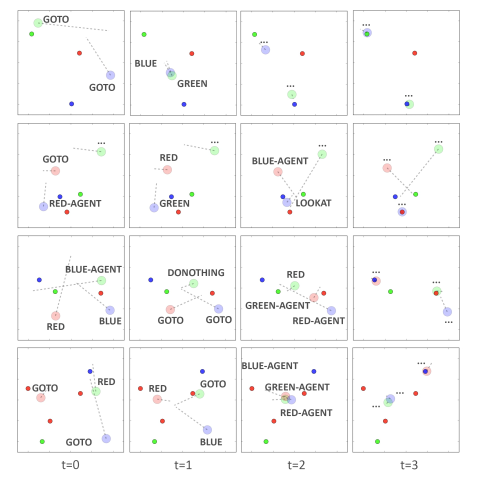
\includegraphics[width=6in]{figure4.png}
	\caption{随时间显示的环境中典型事件序列的集合。每一行都是独立。大圆圈代表代理人,小圆圈代表地标。通信符号显示在发出声音的代理旁边。选择抽象通信符号的标签纯粹是为了可视化和…表示不发出信号符号。}\label{fig:通信符号可视化}
\end{figure}


\section{语法结构}
我们观察到代理人发出的符号流产生的一种新的句法结构。训练后只有两个代理有多个地标的环境
和行动,我们观察每个人的符号形成地标,颜色和每种动作类型。 一个典型的通用和物理代理配置显示
如图4,也是如下:
\par 
\   Green Agent: GOTO, GREEN, ...
\par 
\	Blue Agent: GOTO, BLUE, ...
\par 
抽象符号的标签完全由我们选择可解释性和可视化,对训练没有意义。尽管最近有关于解释连续机器语言的工作(Andreas、Dragan和Klein2017年),我们符号词汇的离散性和小规模使我们可以手动标记符号。有关一致性,请参见补充视频中的结果词汇用法。
\par 
物理环境因素在句法结构中起着一定的作用。动作类型动词goto首先发出,因为动作需要时间在固定环境中完成。当代理接收到goto符号时,它开始向所有标志的质心移动(与所有标志等距),然后在接收到其颜色标识时向特定标志移动。
\par 
当环境配置可以包含三个以上的代理时,代理需要形成相互引用的符号。三种新的符号形式是指从地标颜色中分离出来的代理颜色。典型的对话如图4的第二行和第三行所示。
\par 
\qquad Red Agent: GOTO, RED, BLUE-AGENT, ...
\par
\qquad Green Agent: ..., ..., ..., ...
\par
\qquad Blue Agent: RED-AGENT, GREEN, LOOKAT, ...
\par
当代理是他们的私人目标的对象时,他们不能省略任何话语,在这种情况下,他们可以访问这些信息,并且不需要宣布。在这种语言中,单词的发音没有固定的顺序。每一个符号都有助于句子意义的独立性,类似于许多人类语言中使用的格标记语法策略(Beuls and Steels,2013)。
\par 
由于词汇量大小的惩罚并且不鼓励同义词,因此代理人主要依赖于为每个含义使用一致的符号集 我们展示了聚合流的沟通话语,在图5中显示。
\begin{figure}[htb]
	\centering
	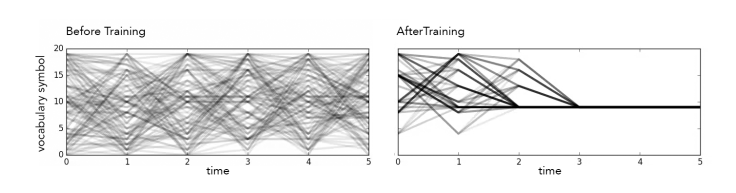
\includegraphics[width=6in]{figure5.png}
	\caption{代理在训练之前和之后随时间发出的通信符号流累积了超过1万个测试试验。}\label{fig:通信符号流累积}
\end{figure}
\par 
在简化的环境配置中,当仅存在一个地标或一种类型的动作时,不形成符号来引用那些概念,因为它们从上下文中是清楚的。


\section{符号词汇用法}
我们发现单词激活计数以确定适当的组成单词计数。在训练早期,在确定适当的有效词汇量大小之前,正在利用大量词汇量来探索通信空间,如图6.在此图中,1x1x3案例指的是具有两个的环境代理和单个动作,只需要传达三个具有里程碑意义的身份之一。1x2x3包含两种类型的操作,3x3x3案例包含三个需要显式引用的代理。

\section{对不可见的配置的推广}
分散执行策略的一个优点是训练有素的代理可以放入任意大小的组中并且仍然可以合理地运行。 当环境中具有相同颜色标识的其他代理程序时,如果引用相同颜色的所有代理程序将执行相同的任务。 此外,当要求特定颜色的代理执行两个冲突的任务(例如被两个不同的代理人要求转到两个不同的地标)时,他们将执行分配给他们的冲突目标的平均值。 尽管在训练期间从未见过,但仍会出现这种情况。

\begin{figure}[htb]
	\centering
	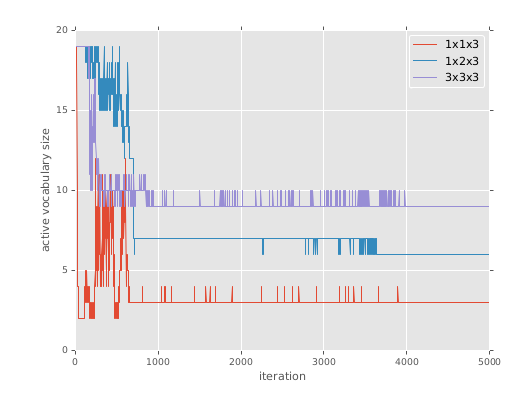
\includegraphics[width=6in]{figure6.png}
	\caption{激活单词计数在不同的环境训练迭代}\label{fig:不同环境训练迭代}
\end{figure}
由于模块化的观察架构,环境中的地标数量也可以在训练和执行之间变化。 尽管没有在这样的环境中接受过培训,但是代理使用不同数量的地标执行合理的行为。 例如,当存在新颖颜色的干扰者地标时,代理永远不会走向它们。 当存在多个相同颜色的地标时,传达目标的代理仍然会发出具有里程碑意义的颜色(因为目标是其中一个地标的位置)。 然而,接收地标色彩话语的代理朝向相同颜色的所有地标的质心,显示出非常明智的概括策略。 在图4的第四行中示出了这种情况的示例

\section{非语言交流和其他策略}
物理环境的存在还允许除语言使用之外的替代策略来实现
目标。在这组实验中,我们使代理能够观察
其他代理人的位置和注视位置,反过来通过符号话语禁用通信能力。当代理可以观察彼此的凝视时,指示策略形成代理可以通过注视其方向来传达地标位置的位置,接收者正确地解释并移动。当无法观察到其他代理人的凝视时,我们会看到目标发送者代理的行为朝着分配给目标接收者代理的位置移动(尽管没有收到明确的奖励),以便将目标接收者引导到该位置。最后,当目标接收者的部分目标都没有视觉和非口头观察时,我们会观察到目标发送者直接将接收者推送到目标位置的行为。这种策略的例子如图7和补充视频所示。对我们来说,建立一个具有多种语言功能的环境非常重要。

\begin{figure}[htb]
	\centering
	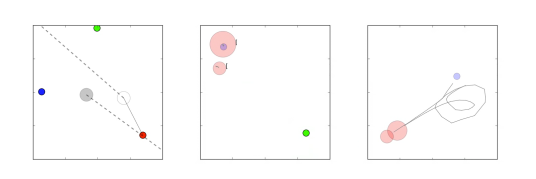
\includegraphics[width=6in]{figure7.png}
	\caption{非言语交流策略的示例,例如指向,引导和推动。}\label{fig:非言语交流策略的示例}
\end{figure}


\section{总结}
我们提出了一种多智能体环境和学习方法,可以从基础经验中产生抽象的组合语言。 这种抽象语言的形成没有任何人类语言使用。 我们调查了代理的环境配置和物理能力的变化如何影响出现的沟通策略。 在未来,我们希望尝试更多的动作,这需要更复杂的语法和更大的词汇表。 我们还希望整合人类语言,以形成与人类使用相容的沟通策略。

\section{致谢}
我们感谢OpenAI团队提供了有用的评论并且富有成效
讨论。 这项工作部分由ONR PECASE资助
N000141612723。

\section{参考}
[Andreas and Klein 2016] Andreas, J., and Klein, D. 2016.
Reasoning about pragmatics with neural listeners and speak-
ers. In Proceedings of the 2016 Conference on Empirical
Methods in Natural Language Processing, EMNLP 2016,
Austin, Texas, USA, November 1-4, 2016, 1173–1182.
$\\$
[Andreas, Dragan, and Klein 2017] Andreas, J.; Dragan, A.;
and Klein, D. 2017. Translating neuralese.
[Austin 1962] Austin, J. 1962. How to Do Things with
Words. Oxford.
$\\$
[Bahdanau, Cho, and Bengio 2014] Bahdanau, D.; Cho, K.;
and Bengio, Y. 2014. Neural machine translation by
jointly learning to align and translate. arXiv preprint
arXiv:1409.0473.
$\\$
[Beuls and Steels 2013] Beuls, K., and Steels, L. 2013.
Agent-based models of strategies for the emergence and evo-
lution of grammatical agreement. PloS one 8(3):e58960.
$\\$
[Bratman et al. 2010] Bratman, J.; Shvartsman, M.; Lewis,
R. L.; and Singh, S. 2010. A new approach to exploring lan-
guage emergence as boundedly optimal control in the face of
environmental and cognitive constraints. In Proceedings of
the 10th International Conference on Cognitive Modeling,
7–12. Citeseer.
$\\$
[Dhingra et al. 2016] Dhingra, B.; Li, L.; Li, X.; Gao, J.;
Chen, Y.-N.; Ahmed, F.; and Deng, L. 2016. End-to-End
Reinforcement Learning of Dialogue Agents for Informa-
tion Access. arXiv:1609.00777 [cs]. arXiv: 1609.00777.
$\\$
[Dosovitskiy and Koltun 2016] Dosovitskiy, A., and Koltun,
V. 2016. Learning to act by predicting the future. arXiv
preprint arXiv:1611.01779.
$\\$
[Durrett, Berg-Kirkpatrick, and Klein 2016] Durrett,
G.;
Berg-Kirkpatrick, T.; and Klein, D. 2016. Learning-based
single-document summarization with compression and
anaphoricity constraints. arXiv preprint arXiv:1603.08887.
$\\$
[Foerster et al. 2016] Foerster, J. N.; Assael, Y. M.; de Fre-
itas, N.; and Whiteson, S. 2016. Learning to Communicate
with Deep Multi-Agent Reinforcement Learning.
$\\$
[Frank and Goodman 2012] Frank, M. C., and Goodman,
N. D. 2012. Predicting Pragmatic Reasoning in Language
Games. Science 336(6084):998.
$\\$
[Gauthier and Mordatch 2016] Gauthier, J., and Mordatch, I.
2016. A paradigm for situated and goal-driven language
learning. CoRR abs/1610.03585.
$\\$
[Golland, Liang, and Klein 2010] Golland, D.; Liang, P.; and
Klein, D. 2010. A game-theoretic approach to generating
spatial descriptions. In Proceedings of the 2010 Confer-
ence on Empirical Methods in Natural Language Process-
ing, EMNLP ’10, 410–419. Stroudsburg, PA, USA: Associ-
ation for Computational Linguistics.
$\\$
[Grice 1975] Grice, H. P. 1975. Logic and conversation. In
Cole, P., and Morgan, J. L., eds., Syntax and Semantics: Vol.
3: Speech Acts, 41–58. San Diego, CA: Academic Press.
$\\$
[Jang, Gu, and Poole 2016] Jang, E.; Gu, S.; and Poole,
B. 2016. Categorical Reparameterization with Gumbel-
Softmax. ArXiv e-prints.
$\\$
[Kirby, Griffiths, and Smith 2014] Kirby, S.; Griffiths, T.;
and Smith, K. 2014. Iterated learning and the evolution
of language. Current opinion in neurobiology 28:108–114.
$\\$
[Kirby 1999] Kirby, S. 1999. Syntax out of Learning: the
cultural evolution of structured communication in a popula-
tion of induction algorithms.
$\\$
[Kirby 2001] Kirby, S. 2001. Spontaneous evolution of lin-
guistic structure-an iterated learning model of the emergence
of regularity and irregularity. IEEE Transactions on Evolu-
tionary Computation 5(2):102–110.
$\\$
[Lake et al. 2016] Lake, B. M.; Ullman, T. D.; Tenenbaum,
J. B.; and Gershman, S. J. 2016. Building machines that
learn and think like people. CoRR abs/1604.00289.
$\\$
[Lazaridou, Peysakhovich, and Baroni 2016] Lazaridou, A.;
Peysakhovich, A.; and Baroni, M. 2016. Multi-agent co-
operation and the emergence of (natural) language. arXiv
preprint arXiv:1612.07182.
$\\$
[Lazaridou, Pham, and Baroni 2016] Lazaridou, A.; Pham,
N. T.; and Baroni, M.
2016.
Towards Multi-
Agent Communication-Based Language Learning. arXiv:
1605.07133.
$\\$
[Littman 1994] Littman, M. L. 1994. Markov games as a
framework for multi-agent reinforcement learning. In Pro-ceedings of the eleventh international conference on ma-
chine learning, volume 157, 157–163.
$\\$
[Maddison, Mnih, and Teh 2016] Maddison, C. J.; Mnih, A.;
and Teh, Y. W. 2016. The concrete distribution: A con-
tinuous relaxation of discrete random variables. CoRR
abs/1611.00712.
$\\$
[Ng 2011] Ng, A. 2011. Sparse autoencoder. CS294A Lec-
ture notes 72(2011):1–19.
$\\$
[Nowak, Plotkin, and Jansen 2000] Nowak, M. A.; Plotkin,
J. B.; and Jansen, V. A. A. 2000. The evolution of syntactic
communication. Nature 404(6777):495–498.
$\\$
[Silver et al. 2016] Silver, D.; van Hasselt, H.; Hessel, M.;
Schaul, T.; Guez, A.; Harley, T.; Dulac-Arnold, G.; Reichert,
D.; Rabinowitz, N.; Barreto, A.; et al. 2016. The pre-
dictron: End-to-end learning and planning. arXiv preprint
arXiv:1612.08810.
$\\$
[Socher et al. 2013] Socher, R.; Perelygin, A.; Wu, J. Y.;
Chuang, J.; Manning, C. D.; Ng, A. Y.; Potts, C.; et al. 2013.
Recursive deep models for semantic compositionality over a
sentiment treebank. In Proceedings of the conference on em-
pirical methods in natural language processing (EMNLP),
volume 1631, 1642. Citeseer.
$\\$
[Steels 1995] Steels, L. 1995. A self-organizing spatial vo-
cabulary. Artif. Life 2(3):319–332.
[Steels 2005] Steels, L. 2005. What triggers the emergence
of grammar? In AISB’05: Proceedings of the Second In-
ternational Symposium on the Emergence and Evolution of
Linguistic Communication (EELC’05), 143–150. University
of Hertfordshire.
$\\$
[Sukhbaatar, Szlam, and Fergus 2016] Sukhbaatar,
S.;
Szlam, A.; and Fergus, R. 2016. Learning multiagent com-
munication with backpropagation. In Advances in Neural
Information Processing Systems 29: Annual Conference on
Neural Information Processing Systems 2016, December
5-10, 2016, Barcelona, Spain, 2244–2252.
$\\$
[Sutskever, Vinyals, and Le 2014] Sutskever, I.; Vinyals, O.;
and Le, Q. V. 2014. Sequence to sequence learning with
neural networks. In Ghahramani, Z.; Welling, M.; Cortes,
C.; Lawrence, N. D.; and Weinberger, K. Q., eds., Advances
in Neural Information Processing Systems 27. Curran Asso-
ciates, Inc. 3104–3112.
$\\$
[Teh 2011] Teh, Y. W. 2011. Dirichlet process. In Encyclo-
pedia of machine learning. Springer. 280–287.
$\\$
[Ullman, Xu, and Goodman 2016] Ullman, T.; Xu, Y.; and
Goodman, N. 2016. The pragmatics of spatial language.
In Proceedings of the Cognitive Science Society.
$\\$
[Vogel et al. 2014] Vogel, A.; Gómez Emilsson, A.; Frank,
M. C.; Jurafsky, D.; and Potts, C. 2014. Learning to reason
pragmatically with cognitive limitations. In Proceedings of
the 36th Annual Meeting of the Cognitive Science Society,
3055–3060. Wheat Ridge, CO: Cognitive Science Society.
$\\$
[Wang, Liang, and Manning 2016] Wang, S. I.; Liang, P.;
and Manning, C. 2016. Learning language games through
interaction. In Association for Computational Linguistics
(ACL).
$\\$
[Winograd 1973] Winograd, T. 1973. A procedural model of
language understanding.


\section{附录:物理状态和动态}
代理的物理状态是由$x = [\mathbf{p} \qquad \dot{\mathbf{p}} \qquad \mathbf{v} \qquad \mathbf{d}]$决定的, $\dot{\mathbf{p}}$是$\mathbf{p}$的速度。$d\in\mathcal{R^3}$是与代理关联的颜色。 地标有相似的状态,但没有凝视和速度成分。单个代理$i$的物理状态转换动态由下式给出:
\par 
$x^t_i = \begin{bmatrix} \mathbf{p} \\ \dot{\mathbf{p}} \\ \mathbf{v} \end{bmatrix}_i^t = \begin{bmatrix} \mathbf{p} + \dot{\mathbf{p}} \Delta t\\ \gamma\dot{\mathbf{p}} + (\mathbf{u}_p + \mathbf{f}(x_{1},...,x_N))\Delta t \\ \mathbf{u}_v \end{bmatrix}_i^{t-1}$
其中$\mathbf{f}(x_{1},...,x_N)$是环境中所有物质与任何障碍物之间的物理相互作用力(如碰撞),$\Delta t$是模拟时间步长(我们使用0.1),$(1 − \gamma)$是阻尼系数(我们使用0.5。
代理的动作空间是$a = [\mathbf{u}_p \qquad \mathbf{u}_v \qquad \mathbf{c}]$
在代理$i$的参考系中对任何$\mathbf{p}_j$的观察是$i\mathbf{P}_j = R_i(\mathbf{P} - \mathbf{P}_i)$,其中$\mathcal{R}_i$是代理$i$的随机旋转矩阵。为每个代理提供私有随机方向可防止在共享坐标系中识别地标(使用诸如最顶层或最左侧的单词)。

%\backmatter
%
%\end{document}
%\endinput
